\documentclass[14pt, a4paper]{article}
\usepackage{indentfirst}
\usepackage{color}
\usepackage[utf8]{inputenc}
\usepackage[english]{babel}
\usepackage{amsmath}
\usepackage{amsfonts}
\usepackage{graphics}
\usepackage{graphicx}
\usepackage{longtable, caption}
\usepackage{makecell}
\usepackage{lscape}
\usepackage{pdflscape}
\usepackage{everypage}
\usepackage{titlesec}
\usepackage{fontspec}
\usepackage{subfig}
\usepackage{caption}
\usepackage{subcaption}
\usepackage{xeCJK}
\usepackage{array}
\usepackage{arydshln}
\usepackage{pgfgantt}
\usepackage[ruled,linesnumbered]{algorithm2e}
\usepackage{adjustbox}
\usepackage{hyperref}
\usepackage{tabularx}
\usepackage{float}
\usepackage{pgfgantt}
\usepackage{xcolor}
\usepackage{enumerate}
\usepackage{algorithmic}
\usepackage{algorithm} 
\usepackage[ruled,vlined,linesnumbered,resetcount]{algorithm2e}
\usepackage{algpseudocode} 
\usepackage{url}
\definecolor{barblue}{RGB}{153,204,254}
\definecolor{groupblue}{RGB}{51,102,254}
\definecolor{linkred}{RGB}{165,0,33}
\renewcommand\sfdefault{phv}
\renewcommand\mddefault{mc}

% Gây lỗi không in đậm được
% \renewcommand\bfdefault{bc}

\setganttlinklabel{s-s}{START-TO-START}
\setganttlinklabel{f-s}{FINISH-TO-START}
\setganttlinklabel{f-f}{FINISH-TO-FINISH}
\sffamily

%\input setbmp
\usepackage{subcaption}
\usepackage[export]{adjustbox}
\usepackage{tikz}
\usepackage{pgfplots}

\newcommand{\Lpagenumber}{\ifdim\textwidth=\linewidth\else\bgroup
  \dimendef\margin=0 %use \margin instead of \dimen0
  \ifodd\value{page}\margin=\oddsidemargin
  \else\margin=\evensidemargin
  \fi
  \raisebox{\dimexpr -\topmargin-\headheight-\headsep-0.5\linewidth}[0pt][0pt]{%
    \rlap{\hspace{\dimexpr \margin+\textheight+\footskip}%
    \llap{\rotatebox{90}{\thepage}}}}%
\egroup\fi}
\AddEverypageHook{\Lpagenumber}%

% Can le van ban
\usepackage[left=3.5cm,right=2cm,top=2cm,bottom=2cm]{geometry}

% Numbering for section, subsection, etc.
\renewcommand{\thesection}{\Roman{section}}
\titlespacing{\section}{2pt}{0pt}{2pt}
\titleformat{\section}{\bfseries\large}{\thesection.}{\hspace{0.5em}}{}
\renewcommand{\thesubsection}{\arabic{subsection}}
\titleformat{\subsection}{\bfseries\large}{\thesubsection.}{\hspace{0.5em}}{}

% subsubsbusection
\titleclass{\subsubsubsection}{straight}[\subsection]

\newcounter{subsubsubsection}[subsubsection]
\renewcommand\thesubsubsubsection{\thesubsubsection.\arabic{subsubsubsection}}
\renewcommand\theparagraph{\thesubsubsubsection.\arabic{paragraph}} % optional; useful if paragraphs are to be numbered

\titleformat{\subsubsubsection}
  {\normalfont\normalsize\bfseries}{\thesubsubsubsection}{1em}{}
\titlespacing*{\subsubsubsection}
{0pt}{3.25ex plus 1ex minus .2ex}{1.5ex plus .2ex}

\makeatletter
\renewcommand\paragraph{\@startsection{paragraph}{5}{\z@}%
  {3.25ex \@plus1ex \@minus.2ex}%
  {-1em}%
  {\normalfont\normalsize\bfseries}}
\renewcommand\subparagraph{\@startsection{subparagraph}{6}{\parindent}%
  {3.25ex \@plus1ex \@minus .2ex}%
  {-1em}%
  {\normalfont\normalsize\bfseries}}
\def\toclevel@subsubsubsection{4}
\def\toclevel@paragraph{5}
\def\toclevel@paragraph{6}
\def\l@subsubsubsection{\@dottedtocline{4}{7em}{4em}}
\def\l@paragraph{\@dottedtocline{5}{10em}{5em}}
\def\l@subparagraph{\@dottedtocline{6}{14em}{6em}}
\makeatother

\setcounter{secnumdepth}{4}
\setcounter{tocdepth}{4}


% Numbering for label itemization
\renewcommand{\baselinestretch}{1.3}

\usepackage{scrextend}
\changefontsizes{13pt}

\renewcommand{\contentsname}{MỤC LỤC}

\renewcommand{\listfigurename}{DANH SÁCH HÌNH VẼ}

\renewcommand{\listtablename}{DANH SÁCH BẢNG}

\renewcommand{\tablename}{Bảng}

\renewcommand{\figurename}{Hình}

\usepackage{textcomp}
\usepackage{listings,multicol}
%\usepackage{minted}      % (requires -shell-escape)
\usepackage{xcolor}
\usepackage{filecontents}

% Code highlight
\usepackage{listings} %code highlighter
\usepackage{color} %use color
\definecolor{mygreen}{rgb}{0,0.6,0}
\definecolor{mygray}{rgb}{0.5,0.5,0.5}
\definecolor{mymauve}{rgb}{0.58,0,0.82}
 
%Customize a bit the look
\lstset{ %
    backgroundcolor=\color{white}, % choose the background color; you must add 
    basicstyle=\footnotesize, % the size of the fonts that are used for the code
    breakatwhitespace=false, % sets if automatic breaks should only happen at whitespace
    breaklines=true, % sets automatic line breaking
    captionpos=b, % sets the caption-position to bottom
    commentstyle=\color{mygreen}, % comment style
    deletekeywords={...}, % if you want to delete keywords from the given language
    escapeinside={\%*}{*)}, % if you want to add LaTeX within your code
    extendedchars=true, % lets you use non-ASCII characters; for 8-bits encodings only, does not work with UTF-8
    frame=single, % adds a frame around the code
    keepspaces=true, % keeps spaces in text, useful for keeping indentation of code (possibly needs columns=flexible)
    keywordstyle=\color{blue}, % keyword style
    % language=Octave, % the language of the code
    morekeywords={*,...}, % if you want to add more keywords to the set
    numbers=left, % where to put the line-numbers; possible values are (none, left, right)
    numbersep=5pt, % how far the line-numbers are from the code
    numberstyle=\tiny\color{mygray}, % the style that is used for the line-numbers
    rulecolor=\color{black}, % if not set, the frame-color may be changed on line-breaks within not-black text (e.g. comments (green here))
    showspaces=false, % show spaces everywhere adding particular underscores; it overrides 'showstringspaces'
    showstringspaces=false, % underline spaces within strings only
    showtabs=false, % show tabs within strings adding particular underscores
    stepnumber=1, % the step between two line-numbers. If it's 1, each line will be numbered
    stringstyle=\color{mymauve}, % string literal style
    tabsize=2, % sets default tabsize to 2 spaces
    title=\lstname % show the filename of files included with \lstinputlisting; also try caption instead of title
}
 
\definecolor{darkgray}{rgb}{.4,.4,.4}
\definecolor{purple}{rgb}{0.65, 0.12, 0.82}
 
%define Javascript language
\lstdefinelanguage{JavaScript}{
    keywords={typeof, new, true, false, catch, function, return, null, catch, switch, var, if, in, while, do, else, case, break},
    keywordstyle=\color{blue}\bfseries,
    ndkeywords={class, export, boolean, throw, implements, import, this},
    ndkeywordstyle=\color{darkgray}\bfseries,
    identifierstyle=\color{black},
    sensitive=false,
    comment=[l]{//},
    morecomment=[s]{/*}{*/},
    commentstyle=\color{purple}\ttfamily,
    stringstyle=\color{red}\ttfamily,
    morestring=[b]',
    morestring=[b]"
}
 
\lstset{
    language=JavaScript,
    extendedchars=true,
    basicstyle=\footnotesize\ttfamily,
    showstringspaces=false,
    showspaces=false,
    numbers=left,
    numberstyle=\footnotesize,
    numbersep=9pt,
    tabsize=2,
    breaklines=true,
    showtabs=false,
    captionpos=b
}


\begin{document}

\captionsetup{justification=centering}


\begin{titlepage}
\centerline{\bf \normalsize VIETNAM NATIONAL UNIVERSITY - HO CHI MINH CITY}
\centerline{\bf \normalsize HO CHI MINH CITY UNIVERSITY OF TECHNOLOGY}
\centerline{\bf \normalsize FACULTY OF COMPUTER SCIENCE AND ENGINEERING}
\vspace*{1cm}
\begin{figure}[h!]
	\begin{center}
		
\includegraphics[width=3cm]{image/bku.png}
		\\
		\vspace{.5cm}
		\LARGE \textbf{INTERNSHIP 1}
	\end{center}
\end{figure}

\begin{center}
    \Large Assignment
    \\
    \LARGE \textbf{Machine learning for internet of thing:\\Person mask detector model in edge device} \\
\end{center}

\vspace{3em}

\begin{table}[h]
\begin{tabular}{rrl}
\hspace{2.5 cm} & Lecturer: & \bf PhD. TBD\\
& Students:  & \bf 2270375 - Nguyễn Trung Thuận\\
\end{tabular}
\end{table}

\vspace{2.5em}

\vfill
\begin{center}
	{\normalsize Ho Chi Minh city - November 2023}
\end{center}
\end{titlepage}


\newpage

\thispagestyle{empty}

% \input{components/loicamdoan_camon}
% \input{components/tom_tat}
\newpage

%\addtocontents{toc}{\protect\thispagestyle{empty}}
\thispagestyle{empty}
\tableofcontents
\thispagestyle{empty}
\newpage
\thispagestyle{empty}
\listoffigures
\thispagestyle{empty}
\newpage

\setcounter{page}{1}

\newpage
\section{Introduction}
\subsection{Machine Learning Introduction}
Machine learning is an innovative application of artificial intelligence (AI) that empowers systems to learn and improve from experience autonomously without explicit programming. 

The learning process begins by observing or obtaining data, such as examples, direct experiences, or instructions, to identify patterns within the data and make informed decisions based on the provided examples. The ultimate goal is to enable computers to learn automatically, free from human intervention, and adapt their actions accordingly.

\subsubsection{Machine Learning algorithm}
\begin{itemize}
\item\textbf{Supervised Machine Learning: }This approach involves leveraging labeled examples from past data to predict the outcome of future events [2]. By analyzing a known training dataset to extract patterns and learn from it, the learning algorithm creates a model to generate predictions about output values. With sufficient training, the system can provide accurate predictions for new inputs. It can also compare its outputs with the correct ones to identify errors and adjust the model accordingly.
\begin{center}
    \begin{figure}[!htp]
        \centering
        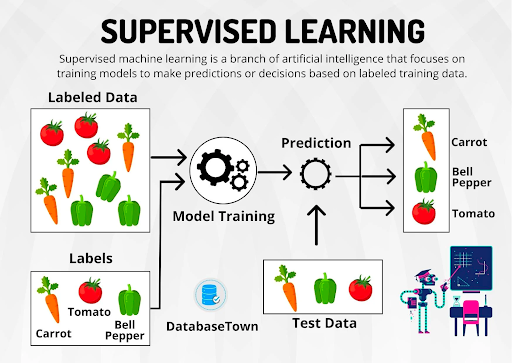
\includegraphics[width=0.8 \textwidth]{image/supervised_learning.png}
        \caption{Supervised learning}
        \label{subsection}
    \end{figure}
    \end{center}
\item\textbf{Unsupervised Machine Learning: } In scenarios where training data lacks labels or classification, unsupervised learning comes into play [3]. This approach focuses on inferring hidden structures within unlabeled data to develop a function that describes the data. While this method does not aim to determine specific outputs, it explores the data to uncover valuable insights and patterns.
\newline
For example (fig 1.2), the algorithm can extract the similar properties of fruits within a bag and group fruits with similar properties into different bags (same color or similar shape)

\begin{center}
    \begin{figure}[!htp]
        \centering
        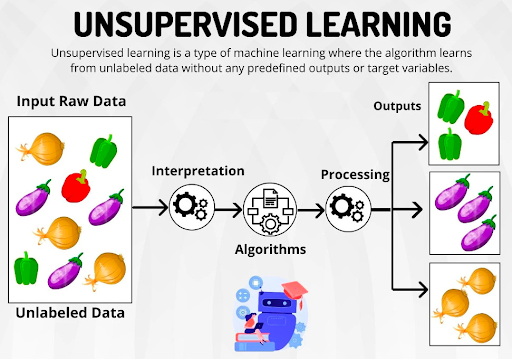
\includegraphics[width=0.8 \textwidth]{image/unsupervised_learning.png}
        \caption{Unsupervised learning}
        \label{subsection}
    \end{figure}
    \end{center}

\item\textbf{Semi-supervised machine learning:} Combining aspects of both supervised and unsupervised learning. This approach utilizes a mix of labeled and unlabeled data for training [4]. Typically, an algorithm works on a small amount of labeled data and a larger pool of unlabeled data. By incorporating this hybrid approach, learning accuracy can significantly improve. Also, obtaining labeled data is expensive and time-consuming, as the model can leverage the large pool of unlabeled data to improve its performance
\begin{center}
    \begin{figure}[!htp]
        \centering
        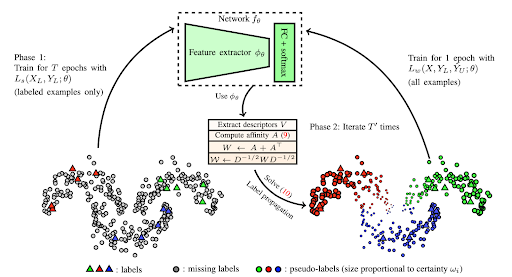
\includegraphics[width=0.8 \textwidth]{image/semi_supervised.png}
        \caption{semi-supervised learning}
        \label{subsection}
    \end{figure}
\end{center}

\item\textbf{Reinforcement learning:} This learning method involves an interactive process where an agent interacts with its environment, taking actions and receiving rewards [5]. Reinforcement learning is characterized by trial and error in making decisions and acquiring rewards. This approach enables machines and software agents to determine the optimal behavior within a specific context, maximizing their performance. Simple reward feedback guides the agent's learning process, known as the reinforcement signal. When combined with AI and cognitive technologies, machine learning becomes a powerful tool for processing vast amounts of information, yielding faster and more accurate results to identify the most profitable opportunities or potential risks. Reinforcement learning is commonly used in areas such as robotics, game-playing, and autonomous systems.
\begin{center}
    \begin{figure}[!htp]
        \centering
        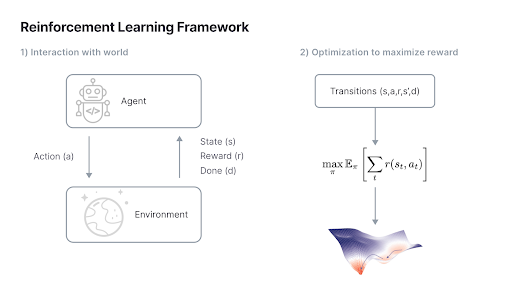
\includegraphics[width=0.8 \textwidth]{image/reinforcement_learning.png}
        \caption{Reinforcement learning}
        \label{subsection}
    \end{figure}
\end{center}
\end{itemize}

\subsection{Machine Learning in Everyday Applications}
\subsubsection{Virtual Personal Assistants}
Virtual personal assistants like Siri, Alexa, and Google Now have become popular examples of AI-driven applications. These assistants provide information and perform tasks when prompted using voice commands. By leveraging machine learning, they refine the information they provide based on user interactions and preferences. 
These assistants are integrated into platforms like Amazon Echo, Google Home, and smartphone software like Samsung Bixby.
\subsubsection{Predictive in communication}
Machine learning plays a crucial role in various aspects of communication. Traffic predictions rely on data from GPS navigation services to generate real-time traffic maps (for example, Google Maps) [6]. 
Machine learning algorithms can estimate areas prone to congestion by analyzing patterns and historical data. Online transportation networks also utilize machine learning to optimize routes, minimize detours, and predict demand, enhancing the efficiency and cost-effectiveness of shared mobility services [7].

\subsubsection{Video surveillance}
Machine learning revolutionizes video surveillance systems by enabling AI-powered detection of potential criminal activities. These systems can identify unusual behaviors, such as prolonged motionlessness or stumbling, and alert human attendants to prevent incidents. 
By continuously learning from data, machine learning enhances the accuracy and effectiveness of video surveillance, improving overall security [8].
\subsubsection{Social media services}
Machine learning underpins various features in social media platforms, enhancing user experiences and personalization. Examples include "People You May Know" recommendations, where machine learning analyzes user connections, profile visits, and shared interests to suggest potential friends. 
Face recognition algorithms leverage machine learning to identify and tag individuals in photos. Additionally, machine learning powers computer vision techniques that identify objects in images and recommend related content [9],
\subsubsection{Recommendation System}
Machine learning is instrumental in recommendation systems used by streaming platforms, e-commerce websites, and social media platforms. 
These systems analyze user preferences, browsing history, and behavior to suggest personalized content, products, or connections. By continuously learning from user feedback and interactions, recommendation systems improve their accuracy and provide tailored recommendations that cater to individual user preferences [10].

\subsection{Internet of Things}
\subsubsection{Introduction}
The Internet of Things (IoT) refers to a networked system where various physical objects are interconnected and accessible via the Internet. These objects, often called "things," can range from individuals with heart monitors to automobiles with sensors. 
Each object is assigned an IP address, enabling them to collect and transmit data over a network without manual intervention. By leveraging embedded technology, these objects can interact with their internal states or the surrounding environment, influencing their decisions. 

Typically, IoT's primary components are devices capable of connecting to the Internet and are divided into Sensors and actuators. Sensors are devices capable of detecting or measuring specific phenomena, collecting related data, and transmitting them to other entities (other IoT devices or application servers in the cloud). 
Some examples of IoT sensors include GPS devices, thermostats, and temperature sensors. To meet the cost-effectiveness requirements of IoT solutions, sensor nodes typically employ small-scale embedded systems, often utilizing 8-bit microcontrollers with limited storage capacity.
This design enables them to operate on battery power for extended periods, sometimes lasting years. Furthermore, a wide range of networking protocols allows sensor nodes to integrate seamlessly into existing infrastructures and diverse operational conditions. This flexibility greatly facilitates the deployment of IoT solutions across various domains [11].

On the other hand, Actuators are physical devices that can execute commands transmitted by a control center or act according to some programmed conditions to create a change in the surrounding environment [12].


\subsubsection{Applications of IoT}
IoT technology enhances mobility services, bolsters public safety, and automates city household systems. Within an area of smart city, one notable application is intelligent transportation, which focuses on optimizing road infrastructure and facilitating efficient route planning for drivers. 
It involves innovative solutions like smart traffic signals and sensors that monitor and manage traffic systems across the road network. By facilitating smoother traffic flow and reducing congestion, these technologies contribute to improved transportation experiences. 
However, the scope of smart city services extends beyond transportation. It encompasses various aspects of urban life, including public safety, environmental sustainability, efficient delivery of municipal services, smart grid systems, and integrating physical infrastructure with the digital realm. [13]

\begin{center}
    \begin{figure}[!htp]
        \centering
        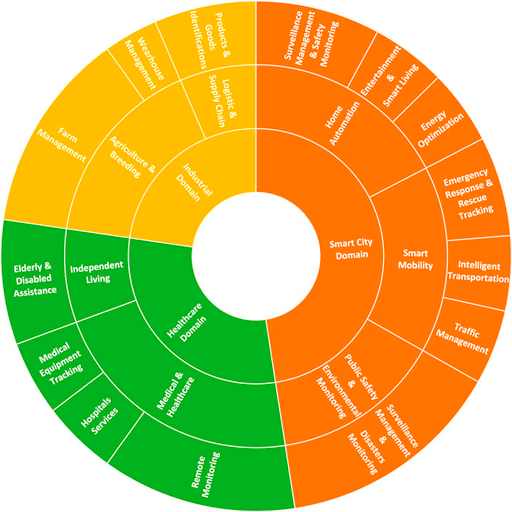
\includegraphics[width=0.8 \textwidth]{image/application_iot.png}
        \caption{Applications of IoT}
        \label{subsection}
    \end{figure}
    \end{center}

Home automation is another section (considered a sub-section of smart city), and control systems have significantly transformed our living environments. They have diverse applications within homes, including entertainment and smart living, surveillance, and safety management. Home automation refers to integrating IoT technology into a standard home environment to provide a secure and comfortable lifestyle. These systems rely on intelligent, self-adaptive mechanisms that analyze and evaluate user behaviors, predict future actions, and interact accordingly.  Home automation systems utilize image detection and facial recognition models embedded in an intelligent control system.
This control system is connected to sensors such as light, motion, water leak, smoke, and CCTV. These devices communicate with each other through a gateway distributed across a home area network. The home control system connects different subsystems collaborating to model user actions and gather environmental information, such as temperature, humidity, noise, visibility, and light intensity, to enhance learning.  For instance, lighting and AC temperature can be controlled and automated based on users' needs and movements within the home environment. Home automation research extends beyond energy optimization and encompasses health monitoring and security measures. 
By leveraging innovative IoT technologies, users can remotely access surveillance cameras within their homes through mobile devices. Additionally, stakeholders can employ door and window sensors to ensure home safety and security from a distance.

IoT has also expanded its application to the industrial sector. Industrial IoT harnesses the capabilities of IoT technology in the business and economic sectors to automate previously complex manual operations, meeting consumer demands while reducing production costs. Various industrial domains, including warehouse operations, logistics services, supply chain management, and agricultural breeding, can benefit from machine-to-machine (M2M) intercommunication, facilitating optimal industrial operations. For example, the application of communicating sensors in agricultural systems. 

\begin{center}
    \begin{figure}[!htp]
        \centering
        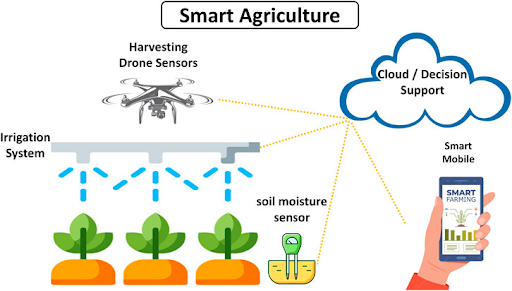
\includegraphics[width=0.8 \textwidth]{image/smart_argi.png}
        \caption{2.2 Smart agricultural system}
        \label{subsection}
    \end{figure}
    \end{center}
This system utilizes smart agriculture technology to monitor and analyze environmental parameters using sensors such as ZigBee, EnOcean, Z-wave, and ANT, which are specifically designed for soil moisture monitoring and harvesting. These sensors are automated to assess the plant's condition and gather relevant data through an IoT platform. Sensors utilize collected information to take appropriate actions, such as determining the optimal timing for irrigation by consulting a weather forecasting service available in the Cloud. It ensures the efficient utilization of water resources while maintaining crop health.
In the Healthcare domain, IoT also has a wide range of applications. IoT sensors and devices have transformed the landscape of portable and wearable medical devices, expanding their applications from fitness and wellness to medically qualified devices suitable for use in hospitals and healthcare facilities. This shift has facilitated the integration of remote patient monitoring (RPM) in healthcare settings, particularly for patients with chronic diseases. As a result, significant efforts are made to advance RPM systems by leveraging well-established IoT infrastructures and standards in the healthcare domain. These RPM systems aim to match or surpass the performance of existing monitoring and examination methods employed in hospitals and healthcare facilities.  For instance, continuous heart rate monitoring and immediate detection of irregular heartbeats traditionally required patients to be hospitalized or connected to devices like Holter monitors for long-term cardiac diagnosis. 
However, these setups limited patient mobility due to device size and the number of connected wires.

Furthermore, hospitals expended substantial resources on providing long-term cardiac monitoring, which was often unavailable, particularly in low or middle-income countries. 
Remote patient monitoring systems effectively address these challenges and reduce mortality rates associated with chronic diseases such as heart disease and diabetes. IoT platforms and devices have played a significant role in accelerating the development and integration of RPM systems into existing healthcare infrastructures. Consequently, a typical RPM implementation encompasses various services, including but not limited to data acquisition, tracking, communication, automated analysis, diagnoses, and notification systems.

\subsection{Neural Networks & Deep learning}
\subsubsection{Neural Networks & Deep learning introduction}
A neural network is a series of algorithms that aims to discover underlying relationships in a dataset by simulating the functioning of the human brain. Neural networks can adapt to changing input, generating optimal results without redesigning output criteria. 
This concept, rooted in artificial intelligence, is increasingly popular in developing intelligent systems.

In finance, neural networks are utilized in various processes such as time-series forecasting, algorithmic trading, securities classification, credit risk modeling, and constructing proprietary indicators and price derivatives.

Moreover, neural networks have been widely used for image recognition tasks such as object detection, image classification, and facial recognition. In natural language processing, it has shown remarkable performance in various tasks such as language translation, sentiment analysis, and text generation. 
Also, the application of neural networks has been demonstrated in speech recognition, autonomous vehicles, and medical diagnosis. 
The functioning of a neural network resembles that of the human brain's neural network. A "neuron" in a neural network is a mathematical function that collects and categorizes information based on a specific architecture. The network bears similarities to statistical methods like curve fitting and regression analysis [14].

A neural network consists of interconnected layers of nodes, where each node functions as a perceptron, similar to multiple linear regression. The perceptron passes the signal from multiple linear regression through an activation function, which can be nonlinear

In a multi-layered perceptron (MLP), perceptrons are organized into interconnected layers. The input layer receives input patterns, while the output layer provides classifications or output signals corresponding to the input patterns. 
For example, input patterns may consist of technical indicators for security, and potential outputs could be "buy," "hold," or "sell".

Hidden layers in the neural network adjust the input weightings until the network's margin of error is minimized. It is hypothesized that hidden layers extract significant features from the input data that have predictive power for the outputs. This process, known as feature extraction, serves a purpose similar to statistical techniques like principal component analysis [15].
\begin{center}
    \begin{figure}[!htp]
        \centering
        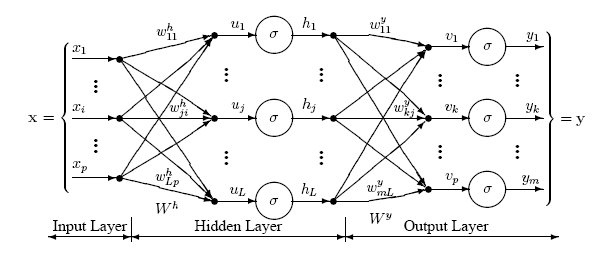
\includegraphics[width=0.8 \textwidth]{image/MLFN_with_weights.jpeg}
        \caption{Multi-layer perceptron}
        \label{subsection}
    \end{figure}
    \end{center}

A Deep Neural Network (DNN) is a type of artificial neural network (ANN) that consists of multiple layers between the input and output layers. The DNN employs various mathematical operations to transform the input into the desired output, accommodating both linear and non-linear relationships.

Deep learning is a specific function within the field of artificial intelligence (AI) that emulates the information processing and pattern recognition capabilities of the human brain. It falls under the umbrella of machine learning and involves the use of neural networks capable of unsupervised learning from unstructured or unlabeled data. It is also referred to as deep neural learning or deep neural network [15].

\subsubsection{Machine learning vs Deep learning}

\begin{center}
    \begin{figure}[!htp]
        \centering
        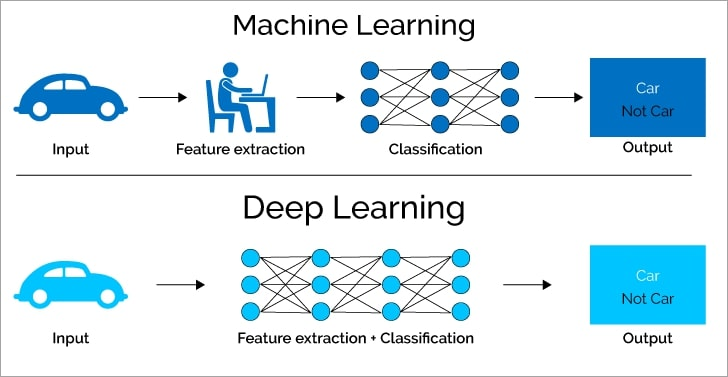
\includegraphics[width=0.8 \textwidth]{image/dnn_vs_ml.png}
        \caption{Deep learning vs Machine learning}
        \label{subsection}
    \end{figure}
    \end{center}

Deep neural networks are characterized by their deeply nested network architectures, typically consisting of multiple hidden layers. These networks employ advanced neurons that utilize operations like convolutions and multiple activations within a single neuron, going beyond the simple activation functions used in traditional artificial neural networks (ANNs). 
It enables deep neural networks to process raw input data and automatically learn representations relevant to the learning task. This capability is commonly referred to as deep learning. In contrast, simple ANNs (such as shallow autoencoders) and other machine learning (ML) algorithms like decision trees are considered part of shallow machine learning as they lack these functionalities. 
While some shallow ML algorithms are inherently interpretable by humans and are considered as white boxes, the decision-making process of most advanced ML algorithms is inherently untraceable unless explicitly explained, making them black boxes.

Deep learning (DL) excels in domains with large and high-dimensional datasets, making deep neural networks outperform shallow ML algorithms in tasks involving text, image, video, speech, and audio data processing. 
However, when dealing with low-dimensional data inputs, especially in scenarios with limited training data availability, shallow ML approaches can still produce superior result, 
which are often more interpretable compared to those generated by deep neural networks [16]. 

\subsubsection{Applications and challenges of AI in Internet of thing}
Several case studies have showcased the successful integration of Internet of Things (IoT) and machine learning technologies in various fields including smart cities such as improving the efficiency of urban services, and enhancing citizens' overall quality of life. 
Deep learning algorithms combined with video analysis have been identified as practical applications in smart cities. 
In one study, researchers developed an IoT system based on deep learning for remote monitoring and early detection of health issues in real time. 
The system exhibited impressive accuracy in identifying heart conditions, achieving a remarkable accuracy rate of 0.982 [17, 18].

However, deploying deep learning methodologies within IoT frameworks presents challenges and limitations. These challenges can be broadly categorized into ethical and privacy implications, scalability and resource constraints, and the ongoing need for research and development.
Integrating deep learning into IoT has significantly advanced security and efficiency in surveillance applications. IoT devices with deep learning capabilities, such as convolutional neural networks, can effectively analyze video streams to detect threats and anomalies, improving real-time monitoring and predictive insights.

Nevertheless, these applications face significant challenges, such as the need for extensive datasets and substantial computational power.
The scalability of deep learning models in the IoT poses a significant concern. IoT devices often have limited computational resources, making it challenging to deploy complex deep-learning models that require substantial data processing capabilities.
It is crucial to optimize these models for deployment on resource-constrained devices, necessitating innovative solutions that strike a balance between the computational demands of deep learning algorithms and the inherent limitations of IoT hardware. [19]


\newpage
\section{Preliminaries}
\subsection{Networks and Node, Community Structure}

\indent In mathematics, graph theory is the study of graphs, which are mathematical structures used to model pairwise relations between objects. A graph (or network) in this context is made up of vertices (also called nodes or points) which are connected by edges (also called links or lines).

A node is a unit of a network that represents an entity, such as a person, a product, a group, or a concept. Edges represent relations between nodes. A graph can be considered as the simplest representation of a complex system, where the vertices are the elementary units of the system and the edges represent their mutual interactions.

The term ”community structure” refers to the composition of a given network, including the number and attributes of nodes, as well as the relationships between them. Community structure is a crucial aspect of complex networks, as it indicates that nodes tend to cluster together into distinct groups or communities.

The term ”community structure” refers to the composition of a given network, including the number and attributes of nodes, as well as the relationships between them. Community structure is a crucial aspect of complex networks, as it indicates that nodes tend to cluster together into distinct groups or communities.

Understanding the community structure of a network can have important implications for many real-world applications, such as predicting the spread of diseases or identifying influential individuals in a social network. Moreover, community detection can also help to reveal underlying patterns and structures in complex systems, providing insights into the organization and behavior of these systems.



Comprehending the community structure of a network carries significant implications for various real-world applications, including forecasting the dissemination of diseases and pinpointing influential individuals within a social network. Furthermore, the process of community detection serves to unveil latent patterns and structures within intricate systems, affording insights into the organizational dynamics and behavioral tendencies inherent in these systems.
\subsection{Community Detection problem}
\indent Communities can be implicit or explicit. Explicit communities are those, in which a grouping is predefined and members joining the group form a community. In this case communities are directly visible, for example whatsapp group. 

\indent Implicit communities on the other hand do not have any predefined classification. We have to analyze the activities of the individuals to form the community. Community detection is used for implicit communities only

\indent Community detection is a fundamental problem in network analysis that aims to identify groups of nodes that are more similar to each other than to the rest of the network. 

\indent One can argue that community detection is similar to clustering. Clustering is a machine learning technique in which similar data points are grouped into the same cluster based on their attributes. Even though clustering can be applied to networks, it is a broader field in unsupervised machine learning which deals with multiple attribute types. On the other hand, community detection is specially tailored for network analysis which depends on a single attribute type called edges. Also, clustering algorithms have a tendency to separate single peripheral nodes from the communities it should belong to. However, both clustering and community detection techniques can be applied to many network analysis problems and may raise different pros and cons depending on the domain.

\indent Community detection is widely used in various fields such as biology, sociology, and marketing to understand social structures, reveal user data within the network, and develop relevant recommendation systems. There are several approaches to community detection, including hierarchical clustering, spectral clustering, modularity maximization, and random walk methods. However, they can be broadly categorized into two types; Agglomerative Methods and Divisive Methods.

\indent In Agglomerative methods, edges are added one by one to a graph which only contains nodes. Edges are added from the stronger edge to the weaker edge. Divisive methods follow the opposite of agglomerative methods. In there, edges are removed one by one from a complete graph.

\indent Ever since the discovery of community structure in real-world networks, a plethora of techniques devoted to their detection has been introduced. The challenge is both theoretical, in proposing a good mathematical definition of what constitutes a community, and computational, in developing good heuristics that can detect communities in a reasonable time.
\subsection{Partitioning quality evaluation}
A common way of investigating the community structure of networks starts with the definition of a quality function, which assigns a score to any network partition. Larger scores correspond to better partitions, and algorithms are created to find the partition with the largest score.

A good community partition of a network should have fewer edges between communities than one would expect by chance. This indicates significant community structure within the network. On the other hand, if the number of edges between groups is what would be expected by chance, it is not evidence of significant community structure. The measure known as modularity quantifies this idea that true community structure corresponds to a statistically surprising arrangement of edges, with fewer edges between groups and more edges within groups than expected by chance.
\subsubsection{Modularity}
Modularity Q is one of the most used measure. The modularity Q is, up to a multiplicative constant, the number of edges falling within groups minus the expected number in an equivalent network with edges placed at random. The modularity can be either positive or negative, with positive values indicating the possible presence of community structure. Thus, one can search for community structure precisely by looking for the divisions of a network that have positive, and preferably large, values of the modularity

The original idea of modularity was given by Newman and Girvan, they have defined modularity Q as:\\
$$Q=\frac{1}{2}\sum_{ij}(A_{ij}-\frac{k_{i}k_{j}}{2m})\delta(\sigma_{i},\sigma{j})$$
Here, m is the number of links, $k_{i}$ is the degree of vertex i, $k_{j}$ is the degree of vertex j, $\sigma_{i}$ is the community to vertex i, $\sigma_{j}$ is the community to vertex j, and $\delta(\sigma_{i}\sigma_{j}) = 1$ if i and j belong to the same community, otherwise it equals to 0.\\
An alternate formulation of this is as a sum over communities:
$$Q=\frac{1}{2m}\sum_{c}(A_{c}-\frac{K_{c}^{2}}{4m})$$
where $m_{c}$ is the number of internal edges (or tatal internal edge weight) of community $c$ and $K_{c} = \sum_{i|\sigma_{i}=c}k_{i}$ is the total (weighted) degree of nodes in community $c$.


\newpage
\section{Project: Speech emotion recognition for edge devices}
\subsection{Motivation}
Human vocal language is an interesting topic that has inspired researchers to explore speech communication with machines for a long time. Various applications, such as smartphone assistants, speech-to-text converters, and voice-operated machines, have been developed in this domain.
However, catching up with human speech is not enough. By enabling machines to recognize and understand human emotions, we can enhance their ability to comprehend us more effectively.

Speech emotion recognition (SER) is a subfield of speech recognition that aims to classify a human speaker's emotional state. It is vital in this domain as it empowers machines to identify and respond to human emotions. Its applications span multiple fields, including safety, entertainment, and biomedicine. 
An exemplary use case is automatic call assistance systems, where understanding customer emotions is vital for providing appropriate service. By discerning emotions, such systems can redirect calls from angry or dissatisfied customers to human agents, ensuring personalized assistance.
In web-based movies and computer tutorials, SER can enhance the viewer's experience by adapting content based on their emotional state [25]

\begin{center}
    \begin{figure}[!htp]
        \centering
        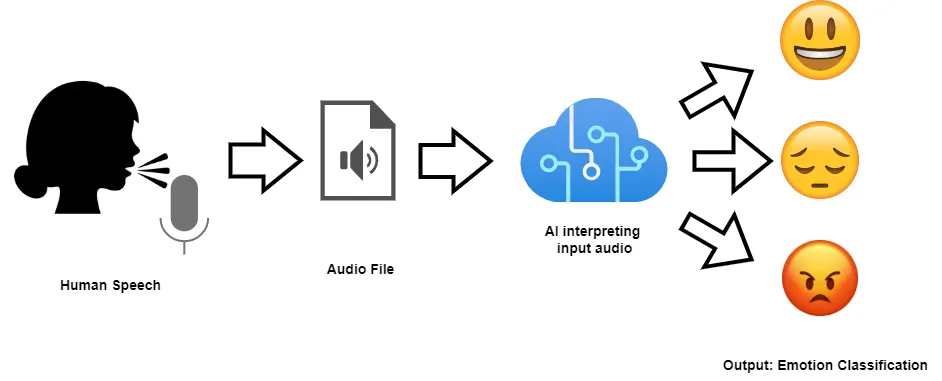
\includegraphics[width=0.8 \textwidth]{image/speech_recognition}
        \caption{Speech recognition system}
        \label{subsection}
    \end{figure}
    \end{center}

In the automotive industry, SER can serve as a safety feature. By monitoring the driver's emotional state, the system can take proactive measures if it detects signs of mental disturbance, ensuring a safer driving experience. 
Additionally, SER holds potential as a diagnostic tool in therapists' hands. Analyzing a patient's speech patterns and emotional expressions can provide valuable insights for assessment and treatment.

In conclusion, integrating speech emotion recognition into machine communication opens up a world of possibilities. 
By recognizing and interpreting human emotions, machines can better comprehend and respond to our needs. Whether in customer service, entertainment, automotive safety, or healthcare, SER has the potential to elevate our interactions with machines to a more intuitive and emotionally aware level.

\subsection{Project overview}
\subsubsection{Introduction}
In this project, I aim to build a lightweight speech emotion recognition model and evaluate its expected performance and power consumption 
using Mel Frequency Cepstral Coefficients (MFCC) and Long Short-Term Memory (LSTM) neural networks. Besides utilizing the TensorFlow Lite framework to compress the model to reduce its memory footprint and computational power requirement, offering the ability to deploy the model on mobiles devices, IoT and wearable devices.
The dataset used for training and evaluation comprises the RAVDESS Emotional speech audio, Toronto emotional speech set (TESS), and Surrey Audio-Visual Expressed Emotion (SAVEE) [1].

\subsubsection{Dataset description}
The RAVDESS dataset (created by Ryerson University's Sensory Communication Group), The TESS dataset (developed by the University of Toronto) and The SAVEE dataset (developed by the University of Surrey) are comprehensive and valuable collections of emotional speech and song recordings.
It consists of audio samples performed by professional actors (male and female artist) who were instructed to portray various emotions, including neutral, happy, sad, angry, fearful, disgust, and surprised.
These datasets serve as valuable resources for training and evaluating models to accurately recognize and classify emotions from speech. [1]

\subsubsection{Preliminary Methodology}
The method employed in this project is based on the work of Sheetal U. Bhandari and Harshawardhan S. Kumbhar. They selected the Long Short-Term Memory (LSTM) architecture and Mel-frequency cepstral coefficients (MFCCs) for the speech emotion recognition (SER) task due to their proven effectiveness in learning from sequences. [26]

For feature extraction, I utilize Mel-Frequency Cepstral Coefficient (MFCC) as it is a popular feature extraction technique for speech recognition [25]. MFCC effectively reduces the computational complexity of the system while enhancing its ability to extract relevant features, including parameters like pitch and energy [3]. By converting the frequency information of the speech signal into a smaller set of coefficients, 
MFCC simplifies the feature extraction process [3]. It represents the short-term power spectrum of sound through a linear cosine transform of a logarithmic power spectrum on a non-linear Mel scale of frequency. [27]

LSTM is a type of recurrent neural network (RNN) that can learn long-term dependencies between time steps of sequence data. It is a popular choice for speech recognition tasks due to its ability to learn from sequences of data since in emotion detection,  it is crucial to take into account the interdependence of each section with the preceding one [26].

Once the standard training and validation pipeline is completed, I convert the model into TensorFlow Lite (TFLite) format, optimizing its size through quantization. Furthermore, I compare the inference time of the quantized model with that of the original model, evaluating the trade-off between model size and inference speed.


\newpage
\section{Experiments}
\subsection{Preprocessing}
The dataset is quite big to handle contain 3 file: \\
    - Books.csv: 271379 records \\
    - Users.csv: 276271 records \\ 
    - \textbf{Ratings.csv: 1149781 records} \\
    
Therefore, we are using the map-reduce technique to split the data in order to fit the computer memory.

The map reduce is using to group and count all pair of books bought by at least 2 users and running on file Ratings.csv. 

Map reduce first phase: 
    % \begin{figure}[H]
    %     \centering
    %     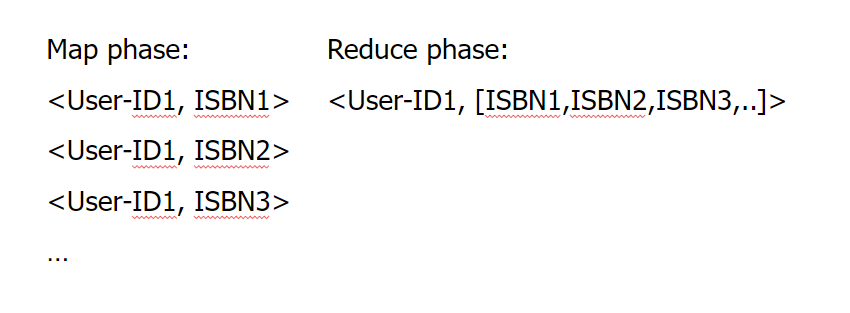
\includegraphics[width=\textwidth]{image/mapreduce 1.png}
    %     \caption{Map reduce first phase find all books were bought by single users}
    % \end{figure}

    \begin{table}[H]
        \centering
        \begin{tabular}{|l|l|}
            \hline
             \textbf{Map phase}       &  \textbf{Reduce phase}\\ \hline
             <User-ID1, ISBN1> & <User-ID1, [ISBN1, ISBN2, ISBN3, ...]> \\
             <User-ID1, ISBN2> & \\
             <User-ID1, ISBN3> & \\ \hline
        \end{tabular}
        \caption{Map reduce first phase find all books were bought by single users}
        \label{tab:my_label}
    \end{table}

Map second phase: 
    % \begin{figure}[H]
    %     \centering
    %     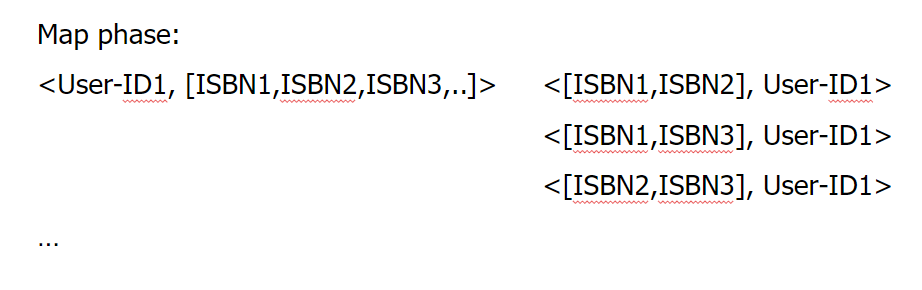
\includegraphics[width=\textwidth]{image/mapreduce 2.png}
    %     \caption{Map phase to find all books pair of book bought by users}
    % \end{figure}

    \begin{table}[H]
        \centering
        \begin{tabular}{|l|l|}
            \hline
             \textbf{Map phase}      &  \\ \hline
             <User-ID1, [ISBN1, ISBN2, ISBN3, ...]> & <[ISBN1, ISBN2], User-ID1> \\
                               & <[ISBN1, ISBN3], User-ID1>\\
                               & <[ISBN2, ISBN3], User-ID1>\\ \hline
        \end{tabular}
        \caption{Map phase to find all books pair of book bought by users}
        \label{tab:my_label}
    \end{table}

Reduce second phase: 
    % \begin{figure}[H]
    %     \centering
    %     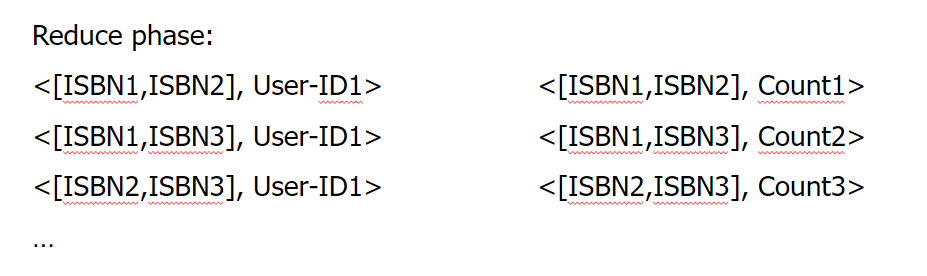
\includegraphics[width=\textwidth]{image/mapreduce 3.png}
    %     \caption{Reduce phase to find all books pair of books and number of users bought it}
    % \end{figure}

    \begin{table}[H]
        \centering
        \begin{tabular}{|l|l|}
            \hline
            \textbf{Reduce phase} &  \\ \hline
             <[ISBN1, ISBN2], User-ID1> & <[ISBN1, ISBN2], Count1> \\
             <[ISBN1, ISBN3], User-ID1> & <[ISBN1, ISBN3], Count2> \\
             <[ISBN2, ISBN3], User-ID1> & <[ISBN2, ISBN3], Count3> \\ \hline
        \end{tabular}
        \caption{Reduce phase to find all books pair of books and number of users bought it}
        \label{tab:my_label}
    \end{table}

% \subsection{Evaluation}


\subsection{Build application}

We built a web application to demonstrate the process of recommendation in book store. Web are built with VueJS as a Frontend and Flask as a framework by Python language programming. Backend is in charge of query similar books and return it to Frontend via Restful api.

\begin{figure}[H]
    \centering
    
\includegraphics[width=0.7\textwidth]{image/technology.png}
    \caption{Technologies used}
\end{figure}

\subsubsection{Build Backend}
\textbf{Flask introduction:} Flask is a micro web framework written in Python. It is classified as a microframework because it does not require particular tools or libraries. It has no database abstraction layer, form validation, or any other components where pre-existing third-party libraries provide common functions.

\textbf{All required libraries:} \\
Create file \textit{requirements.txt}:
\begin{lstlisting}
Flask==2.2.3
Flask-Cors==3.0.10
pandas==2.0.0
networkx==2.8.8
\end{lstlisting}

\textbf{Install all libraries via command:}
\begin{lstlisting}
pip install -r requirements.txt
\end{lstlisting}

\textbf{Run backend locally on port 5000}
\begin{lstlisting}
python main.py
\end{lstlisting}
\subsubsection{Build Frontend}
\textbf{VueJS introduction:} Vue.js is an open-source model–view–viewmodel front end JavaScript framework for building user interfaces and single-page applications. It was created by Evan You, and is maintained by him and the rest of the active core team members

\subsubsubsection{Components}

Include 3 pages
\begin{enumerate}
    \item Homepage: Some categories, and popular items among users
    \begin{figure}[H]
            \centering
            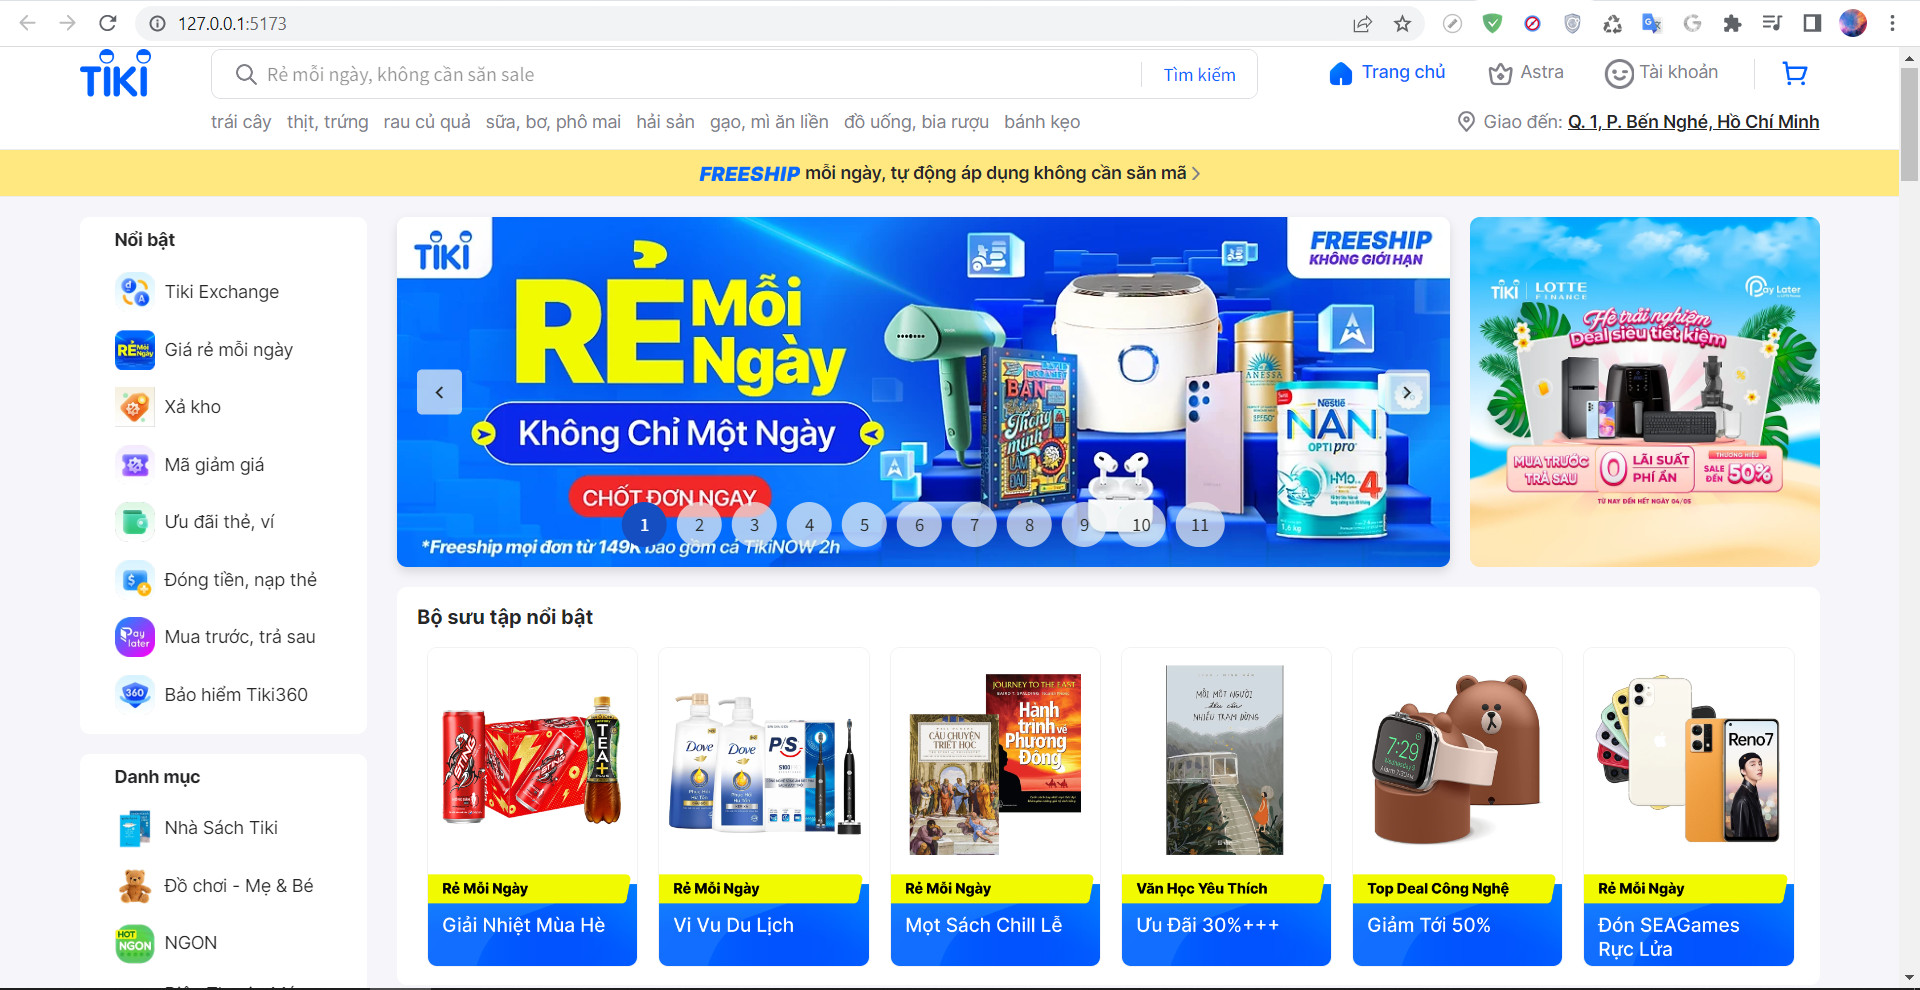
\includegraphics[width=\textwidth]{image/homepage.jpg}
            \caption{Homepage}
        \end{figure}

    \begin{figure}[H]
            \centering
            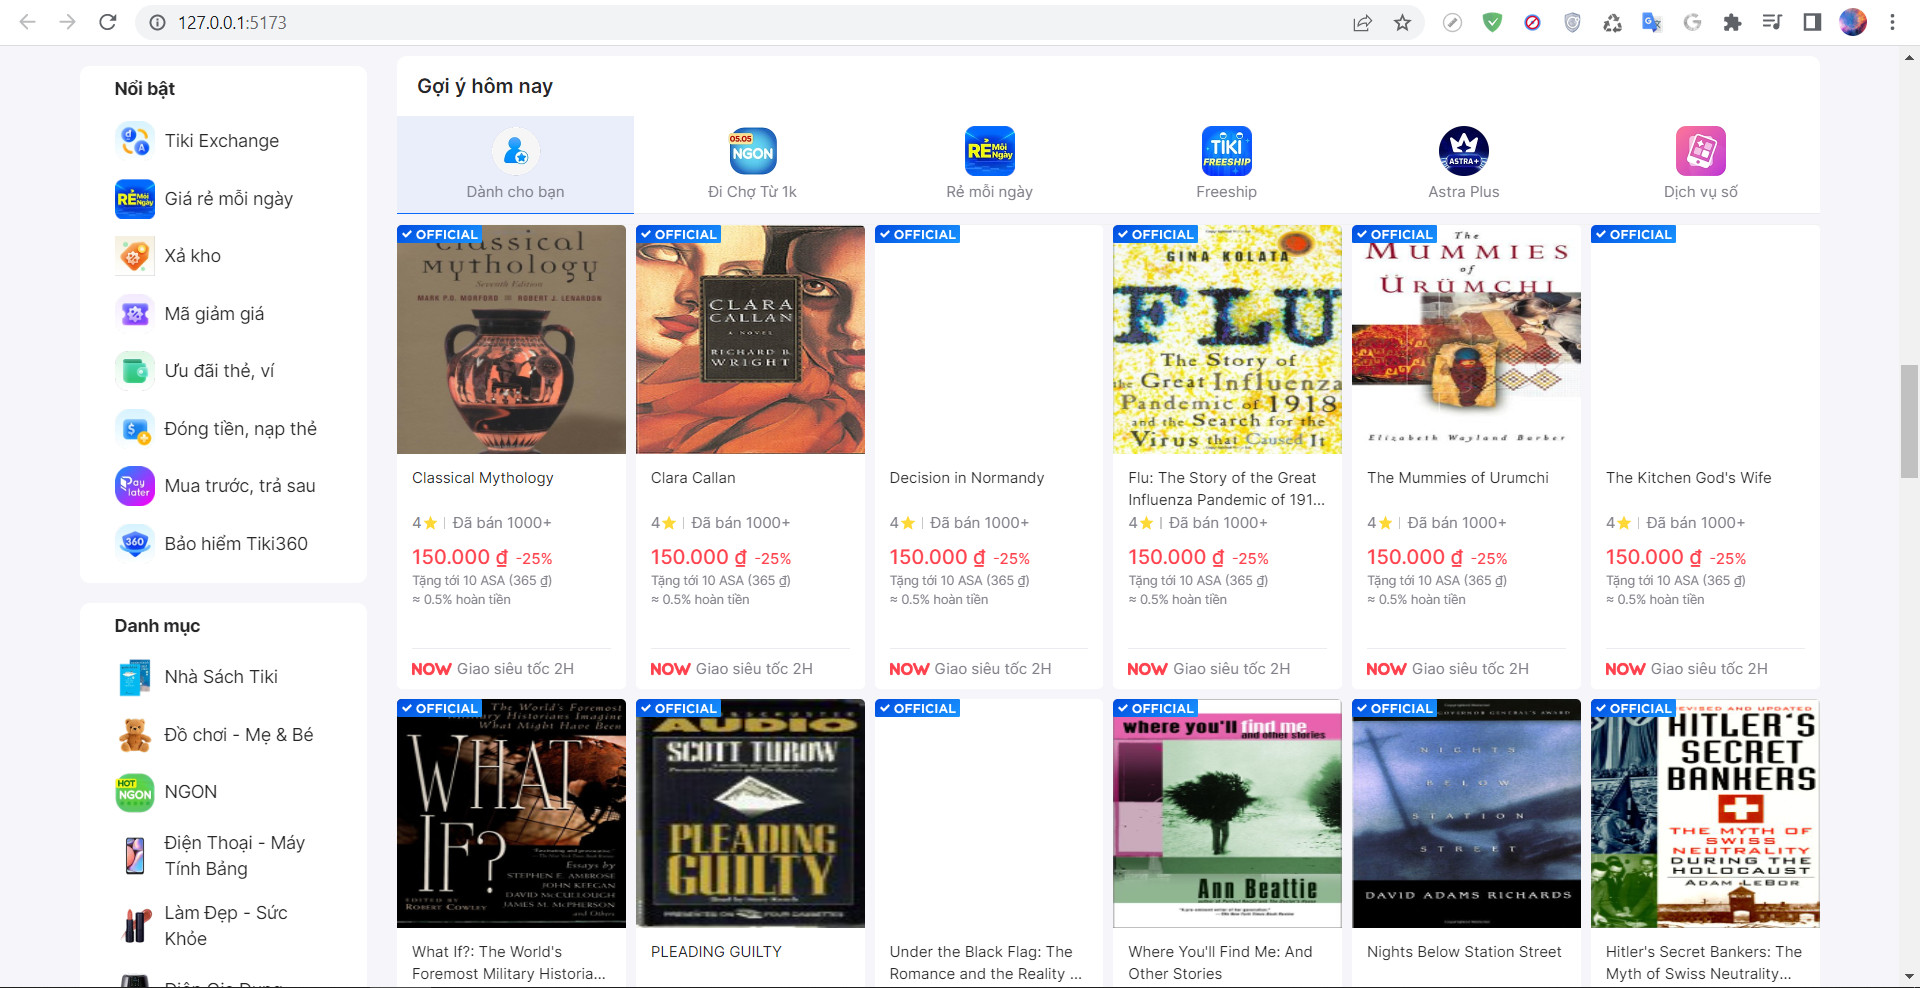
\includegraphics[width=\textwidth]{image/homepage2.jpg}
            \caption{Book category in homepage}
        \end{figure}

    \item Book category page: All books in E-Commerce using pagination.
    \begin{figure}[H]
            \centering
            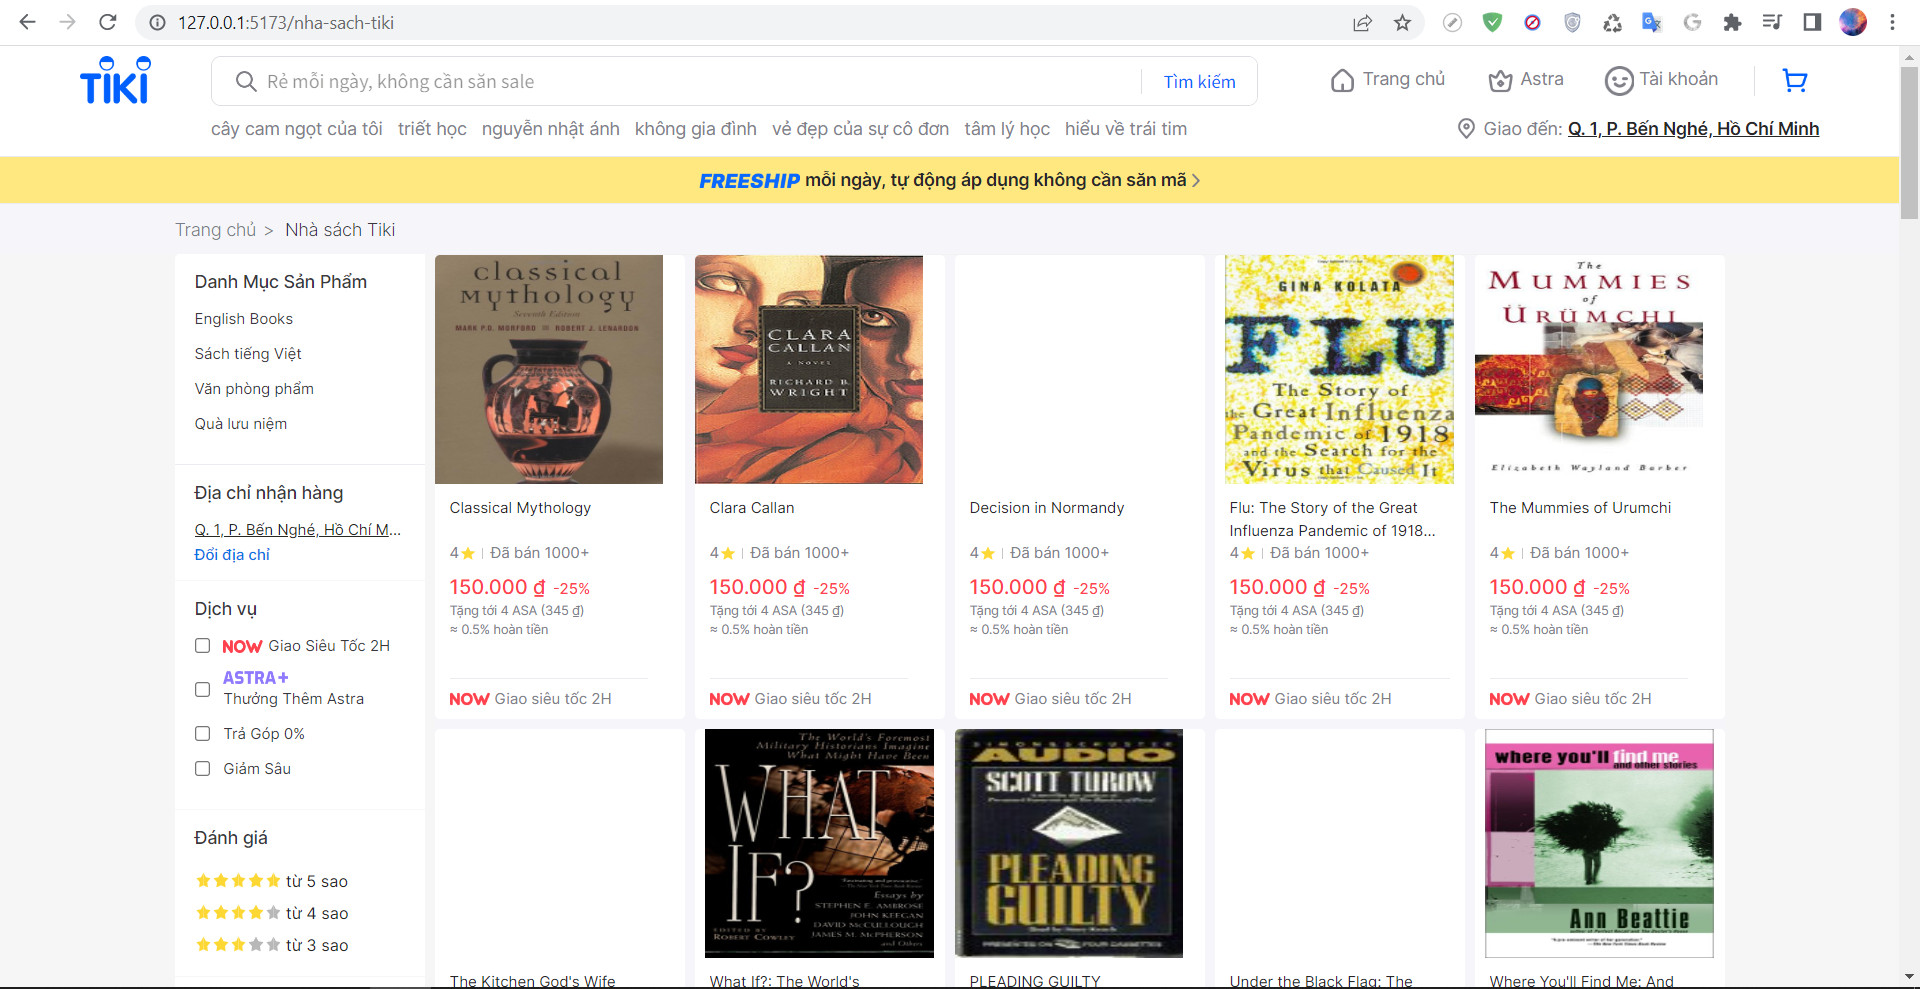
\includegraphics[width=\textwidth]{image/book category.jpg}
            \caption{Book category page}
        \end{figure}

    \item Book detail page: Detail of a book and all similar book using Louvain, Leiden, Girvan Newman.
    \begin{figure}[H]
            \centering
            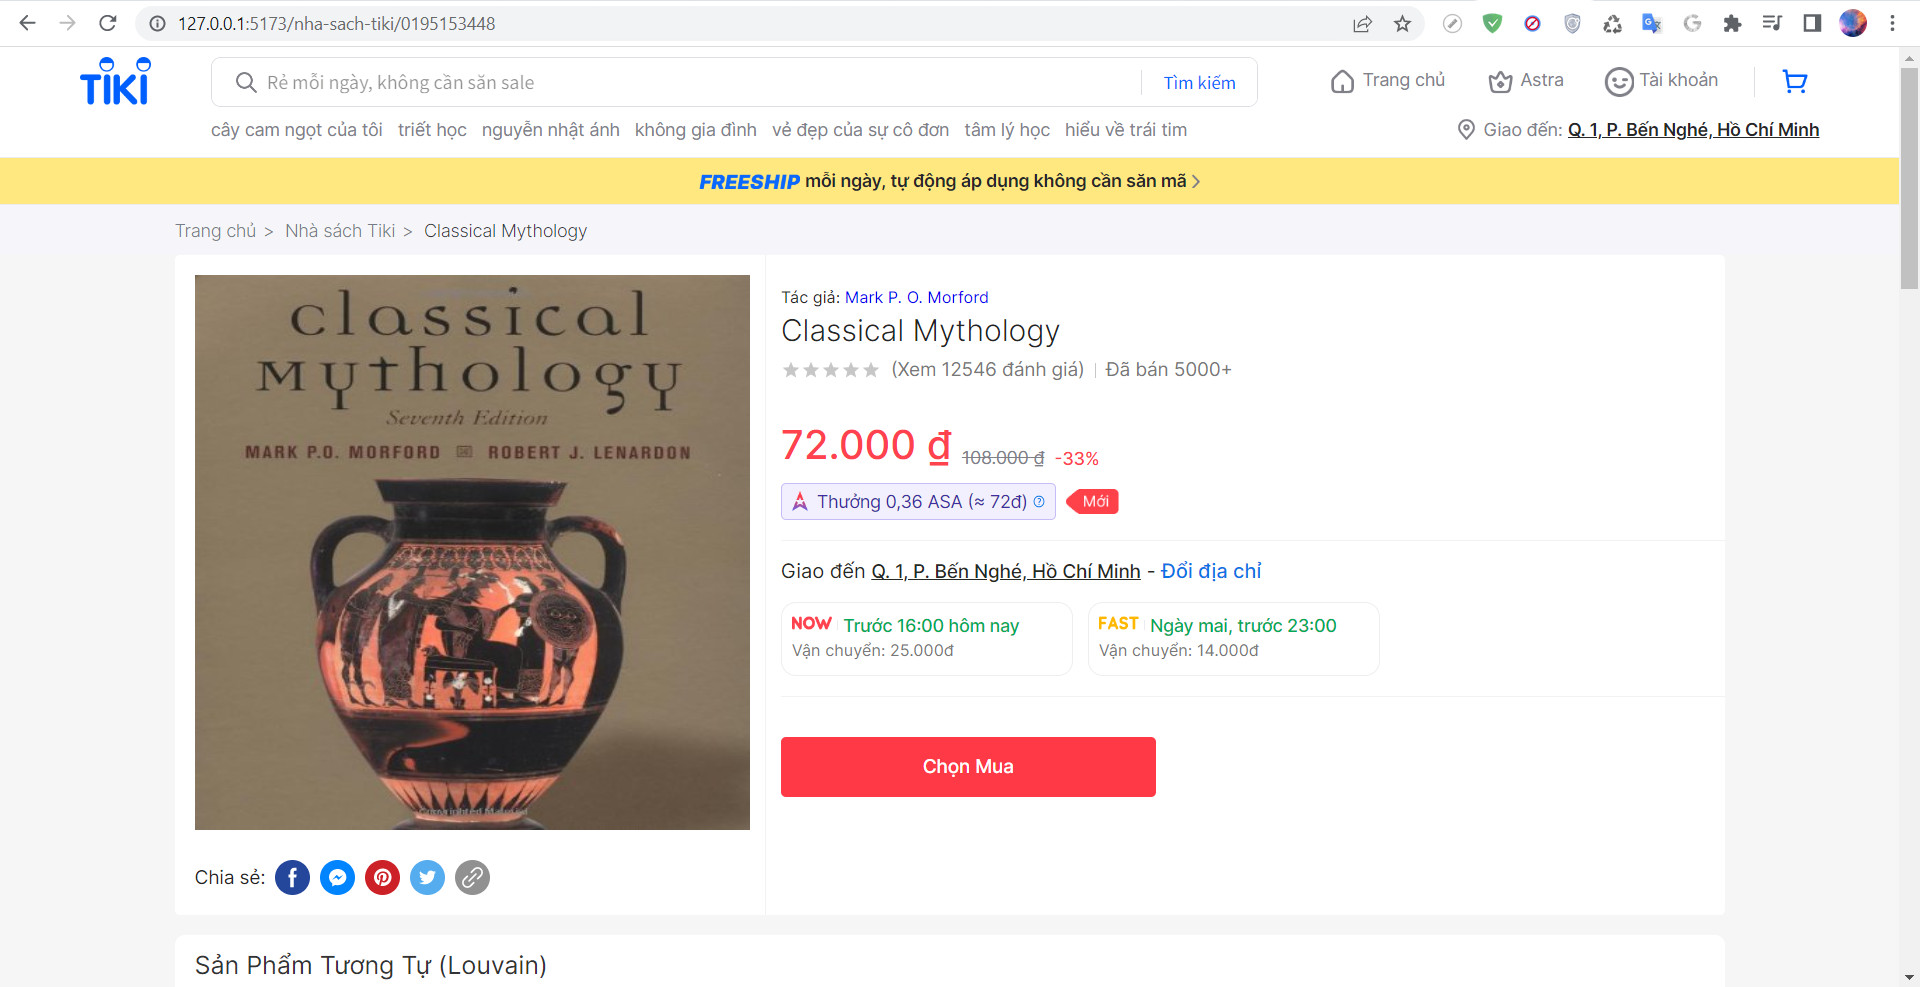
\includegraphics[width=\textwidth]{image/book-detail.jpg}
            \caption{Book detail page}
        \end{figure}

    \begin{figure}[H]
            \centering
            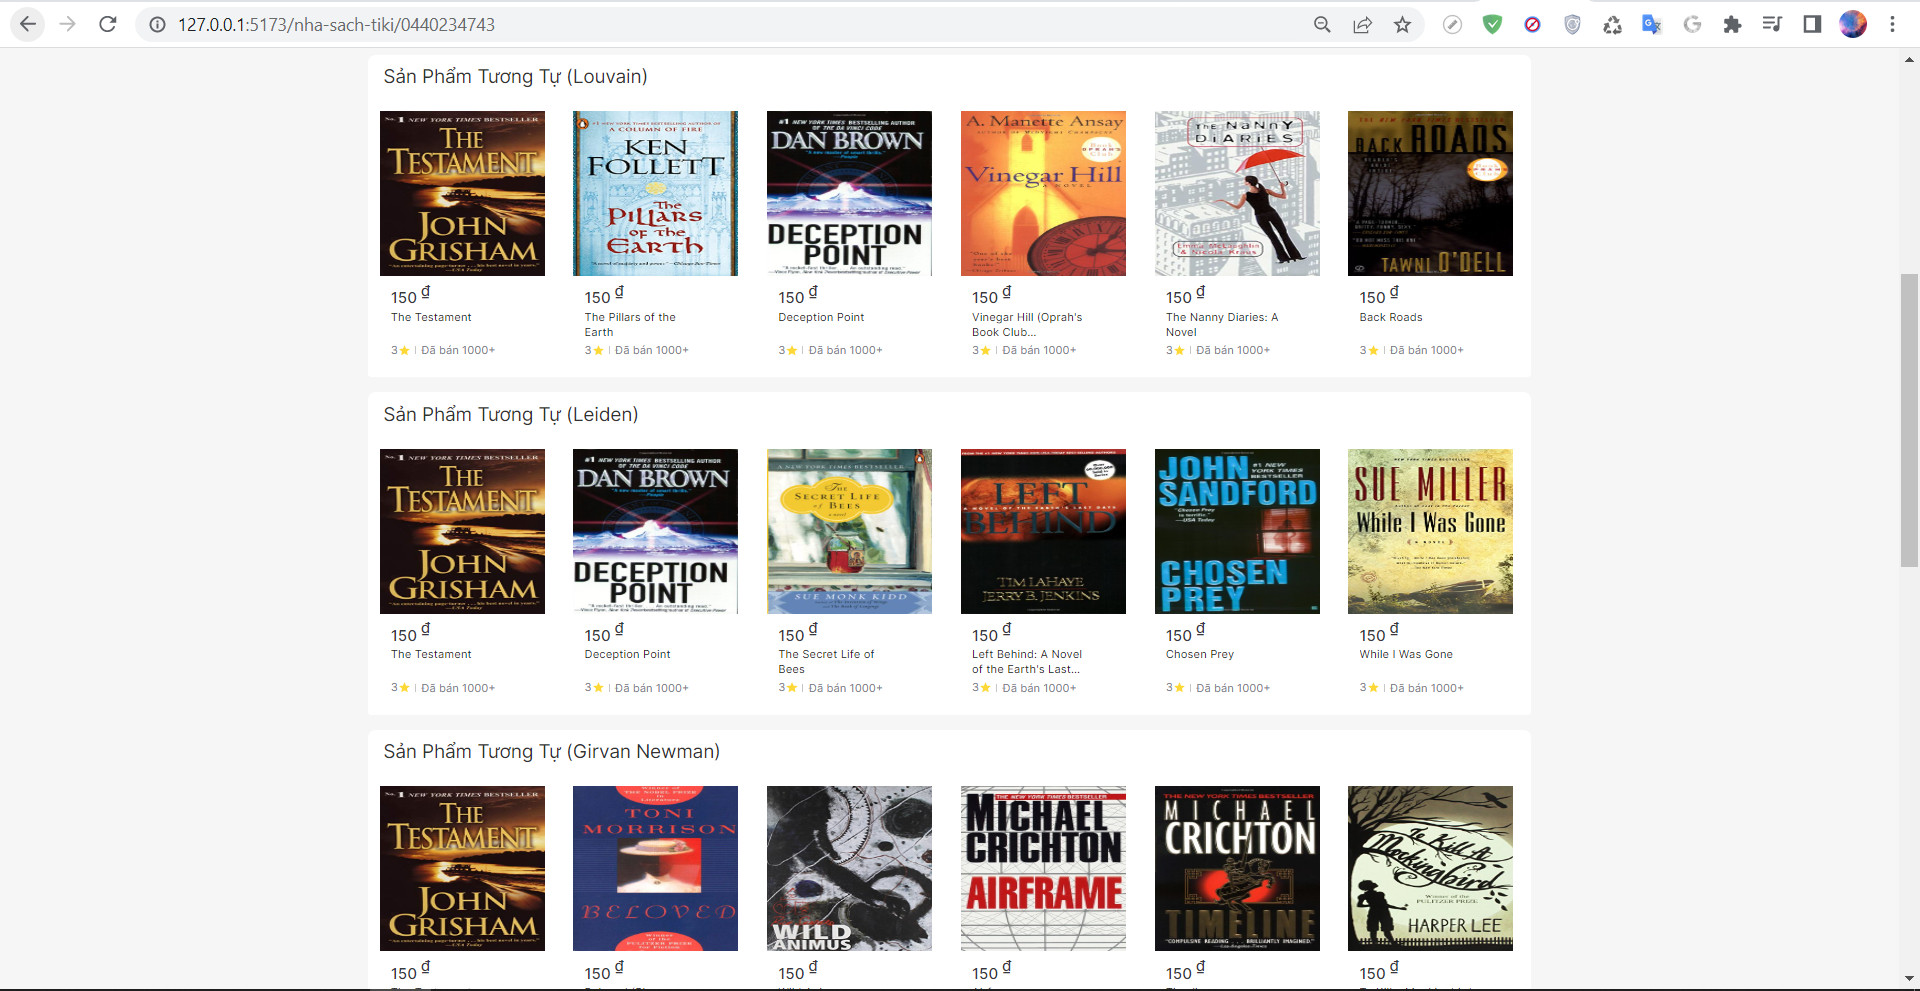
\includegraphics[width=\textwidth]{image/book-detail2.jpg}
            \caption{Book detail page recommendation algorithms}
        \end{figure}
\end{enumerate}

\subsection{Modularity score comparison}
To improve the efficiency of measuring algorithm modularity, we implemented a strategy of dividing the dataset into smaller subsets. Our approach involved selecting the top 500 books that appeared in all book pairs from the previous Map Reduce step. This selection criterion was chosen over random selection from all pairs to avoid generating a sparse graph that would result in significantly lower modularity scores for all three algorithms, making it challenging to measure them accurately.

By ensuring that the selected nodes had the highest number of edges, we aimed to facilitate faster execution of all three algorithms

\begin{figure}[H]
    \centering
    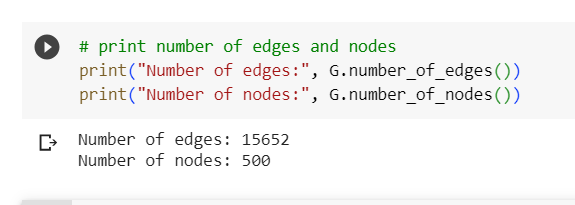
\includegraphics[width=\textwidth]{image/modulairytest.png}
    \caption{Number of edge and node for modularity measurement}
\end{figure}

\begin{figure}[H]
    \centering
    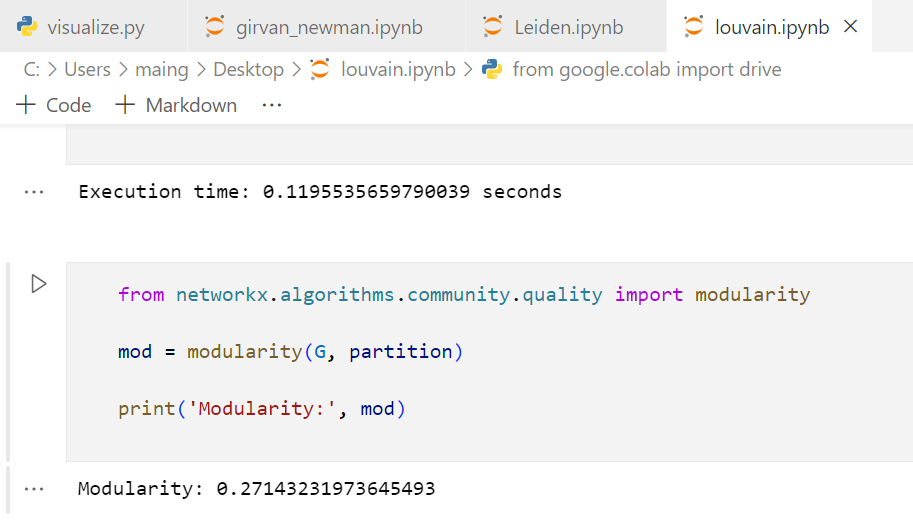
\includegraphics[width=\textwidth]{image/modularity measure louvain.png}
    \caption{modularity measurement for Louvain algorithms}
\end{figure}

\begin{figure}[H]
    \centering
    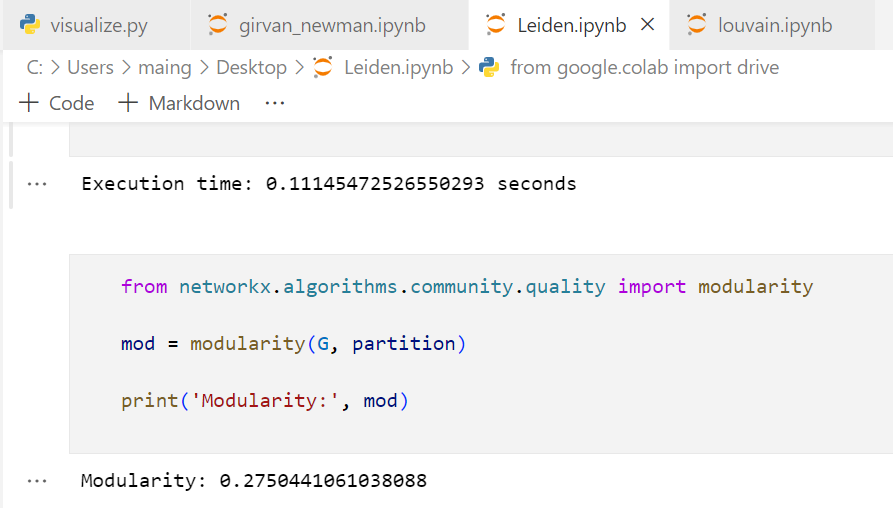
\includegraphics[width=\textwidth]{image/modularity measure leiden.png}
    \caption{modularity measurement for Leiden algorithms}
\end{figure}

\begin{figure}[H]
    \centering
    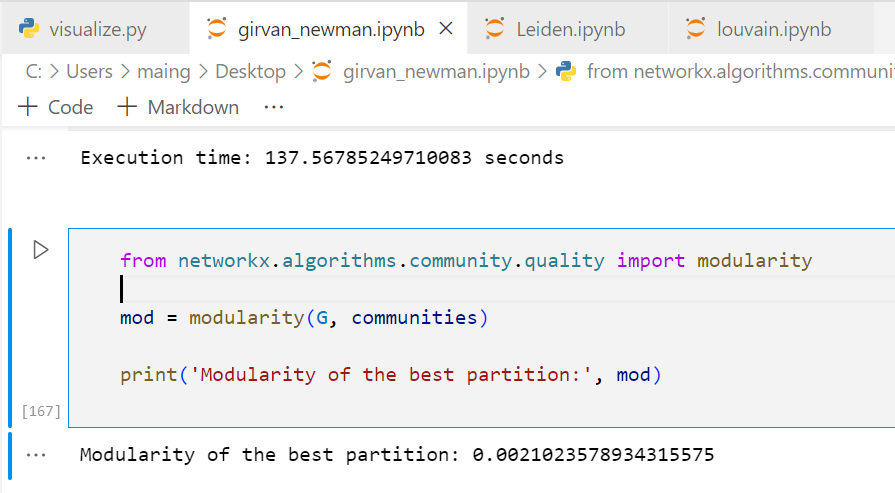
\includegraphics[width=\textwidth]{image/modularity measure girvan.png}
    \caption{modularity measurement for Girvan Newman algorithms}
\end{figure}

Louvain: The Louvain algorithm is recognized for its ability to generate community partitions with high modularity scores. Its iterative optimization process helps identify dense subgraphs and optimize modularity locally and globally.

Leiden: The Leiden algorithm slightly higher score than Louvain.

Girvan-Newman: The Girvan-Newman algorithm tends to have a lower modularity score compared to both Louvain and Leiden. This is because its divisive edge removal approach may not capture the community structure as effectively as the other two algorithms in most cases.

\subsection{Time Efficiency comparison}
To improve the efficiency of measuring algorithm modularity, we implemented a strategy of dividing the dataset into smaller subsets. Our approach involved selecting the top 500 books that appeared in all book pairs from the previous Map Reduce step. To ensured that all three algorithms were executed under similar conditions with large input size.

\begin{figure}[H]
    \centering
    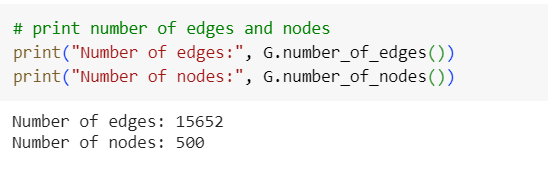
\includegraphics[width=\textwidth]{image/timetest.png}
    \caption{Number of edge and node for time efficiency measurement}
\end{figure}

\begin{figure}[H]
    \centering
    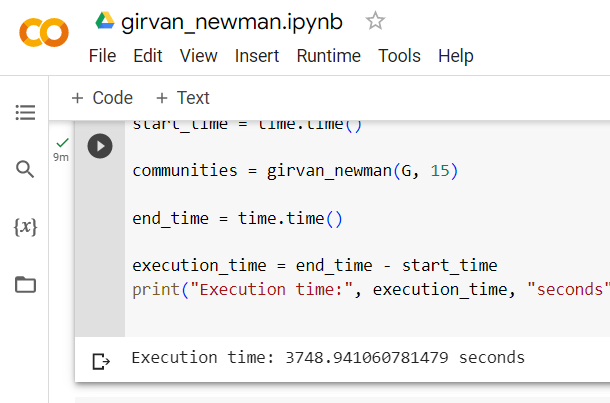
\includegraphics[width=\textwidth]{image/girvantimetest.png}
    \caption{modularity measurement for Girvan Newman algorithms}
\end{figure}

\begin{figure}[H]
    \centering
    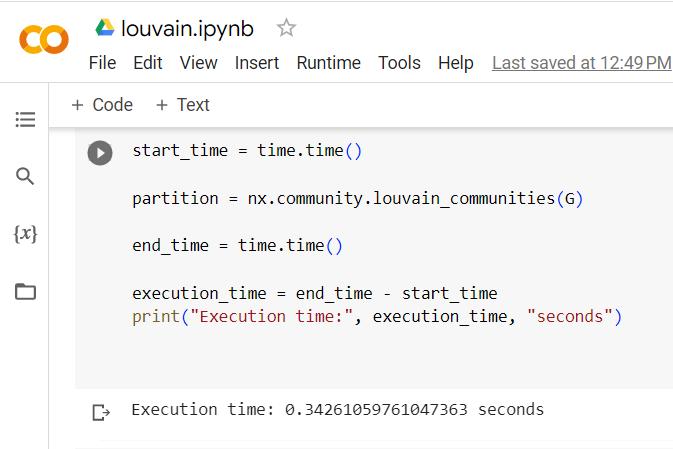
\includegraphics[width=\textwidth]{image/louvaintimetest.png}
    \caption{modularity measurement for Louvain algorithms}
\end{figure}

\begin{figure}[H]
    \centering
    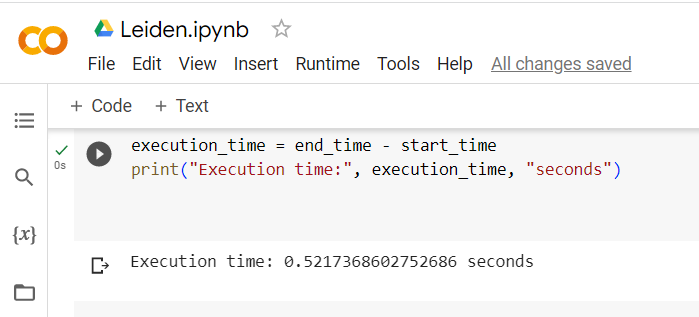
\includegraphics[width=\textwidth]{image/leidentimetest.png}
    \caption{modularity measurement for Leiden algorithms}
\end{figure}

Leiden: The Leiden algorithm is known for its efficiency, particularly in handling large-scale networks. It utilizes techniques such as smart local moving and graph contraction to improve performance.

Louvain: The Louvain algorithm is also efficient and widely used for community detection. It employs a two-phase approach, iteratively optimizing modularity at the local and global levels. However, it can face scalability challenges with very large networks. In this comparison, the execution times of Louvain and Leiden are similar, possibly because the Louvain algorithm has been improved with support from libraries or optimized implementations.

Girvan-Newman: The Girvan-Newman algorithm uses a divisive approach, iteratively removing edges with the highest betweenness centrality to break the graph into communities. This approach is significantly more computationally expensive compared to Louvain and Leiden (3748 seconds), especially for large networks. This is because calculating edge betweenness centrality for all edges can be time-consuming and resource-intensive.

\subsection{Overall comparison}

We have the result of each algorithms: \\

\begin{tabular}{||l|c|c|c||}
    \hline \hline
     & \textbf{Girvan Newman} & \textbf{Louvain} & \textbf{Leiden}  \\ \hline
     \textbf{Modularity} & 0.0021 & 0.2714 & 0.2750\\ \hline 
     \textbf{Time(s)} & 3748.9411 & 0.3426 & 0.5217\\ \hline
     \textbf{Number of} & 12 & 21 & 11\\ 
     \textbf{communities} & & & \\ 
     \hline
     \hline
\end{tabular}
\\
\\
In conclusion, the Louvain and Leiden algorithms generally perform well in terms of modularity score and time efficiency. They are efficient and effective for community detection in various network sizes. However, the Girvan-Newman algorithm, while effective, may not achieve as high modularity scores and much more computationally expensive. It is important to consider the specific characteristics of the network and the desired trade-offs between modularity and runtime when selecting an appropriate algorithm for community detection.


\newpage 
\section{Conclusion}
\subsection{Achievement}

The algorithms that the group used to solve the community search problem for the artist dataset above accomplished the following:

\begin{itemize}
    \item Our team have implemented and runned 3 algorithms (Girvan Newman, Louvain, Leiden) on Python, from that, we can see some comparisions and how they works.

    \item Using the above data clusters, we can suggest similar books to the user while they are seeing the information of the books they want to buy, increasing the diversity of the e-commerce website such as Tiki.

    \item Analyzing the tastes of the readers community in specific clusters to promote better suggestions and apply them to run ads or PR is another strength that this algorithm brings.

    \item Besides, we also build a website to demonstrate our work and its application. The demonstration video of the website is here: \url{https://youtu.be/nnhuGfggjb4}
\end{itemize}

\subsection{Drawback}
Because of the limited research time, the group did not generate many algorithms or make very specific comparisons with the algorithms sought. \\
However, with the above three algorithms,Girvan-Newmana and Louvain, classical algorithms, and Leiden, an improved algorithm widely used today, the group has also made appropriate comparisons of performance and reliability to generalize them.

\subsection{Future work}
The team plans to use more algorithms in the future to get a thorough understanding of the approaches used by businesses and researchers to address problems.

The team also intends to work with more actual data sets in order to fully assess the algorithm’s efficacy and its potential for use in other contexts. This deals with, for instance, developing techniques for providing suggestions or advertising using these data clusters.

\newpage
\section*{References.}
\renewcommand\refname{}
\addcontentsline{toc}{section}{\protect\numberline{}References}%


\begin{thebibliography}{00}


% \bibitem{data-driven-business}
% He, Lifeng, et al. "A linear-time two-scan labeling algorithm." Proceedings of the 2007 IEEE International Conference on Image Processing (ICIP), vol. 5, IEEE, 2007

% \bibitem{data-driven-business}
% Connected-component labeling. Truy cập ngày 15/04/2023\\
% \url{https://en.wikipedia.org/wiki/Connected-component_labeling#One_component_at_a_time}


% \bibitem{data-driven-business}
% The connected-component labeling problem: A review of state-of-the-art algorithms. Truy cập ngày 20/04/2023\\
% \url{https://www.sciencedirect.com/science/article/pii/S0031320317301693#bib0061}
% \end{thebibliography}

\bibitem{Dataset}
Dataset source: \url{https://www.kaggle.com/datasets/ahmedaliraja/customer-rating-data-by-amazon/data}

\bibitem{CommunityStructure}
Lilian Weng, Filippo Menczer & Yong-Yeol Ahn (2013). "Virality Prediction and Community Structure in Social Networks". Last access 26/05/2023\\
\url{https://www.researchgate.net/publication/256188948_Virality_Prediction_and_Community_Structure_in_Social_Networks}

\bibitem{CommunityStructure}
Fabian Nguyen (2021). "Leiden-Based Parallel Community Detection". Last access 26/05/2023\\
\url{https://i11www.iti.kit.edu/_media/teaching/theses/ba-nguyen-21.pdf}

\bibitem{algorithm}
Clauset, A., Newman, M. E., & Moore, C. (2004). Finding community structure in very large networks. ArXiv. 
\url{https://doi.org/10.1103/PhysRevE.70.066111}

\bibitem{louvain}
Blondel, V. D., Guillaume, J., Lambiotte, R., & Lefebvre, E. (2008). Fast unfolding of communities in large networks. ArXiv. 
\url{https://doi.org/10.1088/1742-5468/2008/10/P10008}

\bibitem{LabelPropagation}
Garza, S. E., & Schaeffer, S. E. (2019). Community detection with the Label Propagation Algorithm: A survey. Physica A: Statistical Mechanics and its Applications, 534, 122058. 
\url{https://doi.org/10.1016/j.physa.2019.122058}

\end{thebibliography}

\end{document}
